\documentclass{article}
% translate with >> pdflatex -shell-escape <file>

% This file is used as unit test for pgfplots, copyright by Christian Feuersaenger.
% 
% See
%   http://pgfplots.sourceforge.net/pgfplots.pdf
% for pgfplots.
%
% Any required input files (for <plot table> or <plot file> or the table package) can be downloaded
% at
% http://www.ctan.org/tex-archive/graphics/pgf/contrib/pgfplots/doc/latex/
% and
% http://www.ctan.org/tex-archive/graphics/pgf/contrib/pgfplots/doc/latex/plotdata/

\usepackage{pgfplots}
\pgfplotsset{compat=newest}

\pagestyle{empty}

\begin{document}



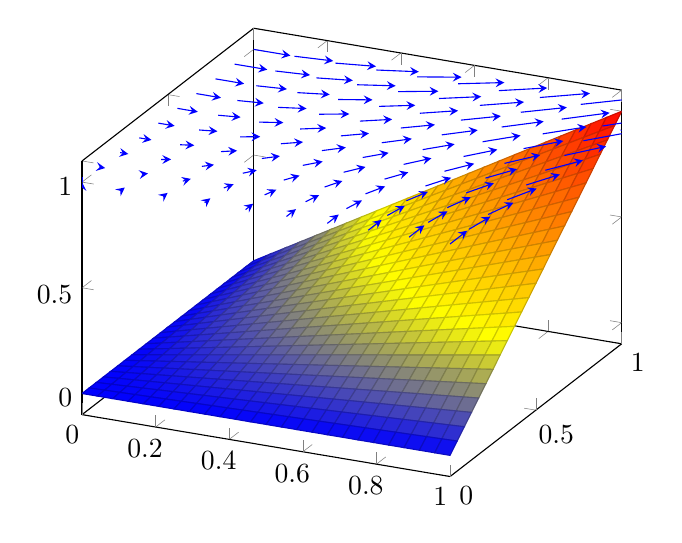
\begin{tikzpicture}
	\begin{axis}[
		domain=0:1,
		xmax=1,
		ymax=1,
	]
		\addplot3[surf] {x*y};
		\addplot3[blue,/pgfplots/quiver,
			quiver/u=0.1*y,
			quiver/v=0.1*x,
			quiver/w value=0,
			-stealth,samples=10] {1};
	\end{axis}
\end{tikzpicture}
\end{document}
